\chapter{Background}
\label{chap:background}

The background necessary for this research includes four main topics. A basic introduction to the safety assessment process is given along with definitions of important artifacts used in the process. Related work gives an overview of pertinent literature in this area of research. The specific modeling language and related tools are described, and lastly, important formal definitions are explained and provided for better understanding of the theoretical contributions of this dissertation.

\section{The Safety Assessment Process and Required Artifacts}
%\subsection{Overview of the Process and Its Artifacts}
In order to approve an aircraft for flight through the FAA, one must show compliance with federal safety regulations. Industry has over the decades adopted standards published by the Society of Automotive Engineers (SAE); these include Aerospace Information Reports (AIR) and Aerospace Recommended Practices (ARP). These standards aim to provide an organized and acceptable approach for safety analysis that serves to meet the federal regulations and provides industry with a methodology for safety assessment~\cite{FAA,SAE}. Various artifacts are commonly used in the safety assessment process to show the behavior and functionality of the system in the presence of faults. Often, these artifacts are necessary for certification of the system. One artifact that is important to this research is a fault tree and its related minimal cut sets.

\subsubsection{Fault Tree Analysis and Minimal Cut Sets}
The use of fault trees are common in many safety assessment processes and the ability to generate the cut sets needed for the construction of the fault tree is a useful part of any safety analysis tool. The fault tree is a safety artifact commonly referenced in requirement protocol documents such as ARP4761, ARP4754, and AIR6110~\cite{SAE:ARP4761,SAE:ARP4754A,AIR6110}.

A Fault Tree (FT) is a directed acyclic graph whose leaves model component failures and whose gates model failure propagation~\cite{0f356f05e72f43018211b36f97c8854a}. The system failure under examination is the root of the tree and is called the Top Level Event (TLE). The node types in a fault tree are \textit{events} and \textit{gates}. An event is an occurrence within the system, typically the failure of a subsystem down to an individual component. Events can be grouped into \textit{basic events} which occur independently, and \textit{intermediate events} which occur dependently and are caused by one or more other events~\cite{historyFTA}.  These events model the failure of the system (or subsystem) under consideration. The gates represent how failures propagate through the system and how failures in subsystems can cause system wide failures. The two most common logic symbols used in an FT are the Boolean logic AND-gates and OR-gates. An AND-gate is used when the undesired top level event can only occur when all the lower conditions are true. The OR-gate is used when the undesired event can occur if any one or more of the next lower conditions is true. This is not a comprehensive list of gate types; others include voting, inhibit, or negation gates~\cite{0f356f05e72f43018211b36f97c8854a}.
\begin{figure}[h]
\begin{center}
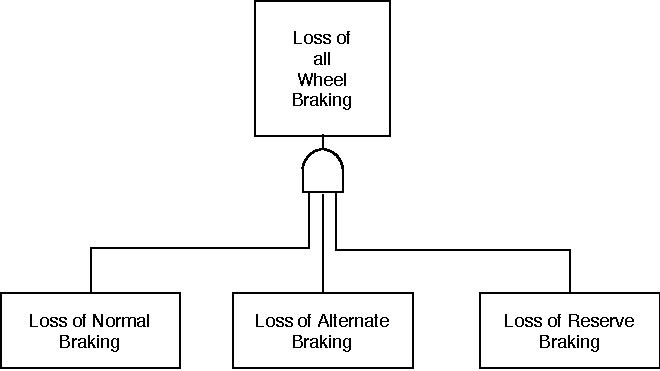
\includegraphics[width=8cm]{images/introFT2.pdf}
\caption{A simple fault tree} \label{fig:introFT}
\end{center}
\end{figure}

Figure~\ref{fig:introFT} shows a simple example of a fault tree based on SAE ARP4761~\cite{SAE:ARP4761}. In this example, the top level event corresponds to an aircraft losing all wheel braking. In order for this event to occur, all of the basic events must occur. This is seen through the use of the AND gate below the top level event. The gates in the fault tree describe how failures propagate through the system. Each gate has one output and one or more inputs. In Figure~\ref{fig:introFT}, the AND gate has three inputs and one output. The leaves of the tree represent the basic events of the system. %and 
In the case of this fault tree, these three events are also the Minimal Cut Sets (MinCutSets) for this top level event. A MinCutSet is the minimal set of basic events that must occur together in order to cause the TLE to occur. Generating and analyzing these MinCutSets is important to FTA and has been an active area of interest in the research community since fault trees were first described in Bell Labs in 1961~\cite{historyFTA,0f356f05e72f43018211b36f97c8854a}. 

There are two main types of fault tree analysis that we differentiate here as \textit{qualitative} analysis and \textit{quantitative} analysis. In qualitative analysis, the structure of the fault tree is considered and the MinCutSets are a way to indicate which combinations of component failures will cause the system to fail. On the other hand, in quantitative analysis the probability of the TLE is calculated given the probability of occurrence of the basic events. 

\subsection{The Traditional Safety Assessment Process}
\label{sec:saProcess}
The traditional safety assessment process at the system level is based on the standards ARP4754A~\cite{SAE:ARP4754A} and ARP4761~\cite{SAE:ARP4761}. It starts with the System level Functional Hazard Assessment (SFHA) examining the functions of the system to identify potential functional failures and classifies the potential hazards associated with them. 

The next step is the Preliminary System Safety Assessment (PSSA), updated throughout the system development process. A key element of the PSSA is a system level Fault Tree Analysis (FTA).  The FTA is a deductive failure analysis to determine the causes of a specific undesired event in a top-down fashion. For an FTA, a safety analyst begins with a failure condition from the SFHA, and systematically examines the system design (e.g., signal flow diagrams provided by system engineers) to determine all credible faults and failure combinations that could cause the undesired event. 

The lack of precise models of the system architecture and its failure modes often forces safety analysts to devote significant effort to gathering architectural details about the system behavior from multiple sources. Furthermore, this investigation typically stops at system level, leaving software function details largely unexplored.

Typically equipped with the domain knowledge about the system, but not detailed knowledge of how the software applications are designed, practicing safety engineers find it a time consuming and involved process to acquire the knowledge about the behavior of the software applications hosted in a system and its impact on the overall system behavior.
Industry practitioners have come to realize the benefits of using models in the safety assessment process, and a revision of the ARP4761 to include Model Based Safety Analysis (MBSA) is under way. %Section \ref{sec:mbsa_appendix_review} provides a comparison of our approach with it.

\subsection{Model-Based Safety Assessment Process Supported by Formal Methods}
\label{sec:saProcess2}
We propose a model-based safety assessment process backed by formal methods to help safety engineers with early detection of the design issues.  This process uses a single unified model to support both system design and safety analysis. It is based on the following steps:

\begin{enumerate}
	\item System engineers capture the critical information in a shared %AADL/AGREE 
	model:  high-level hardware and software architecture, nominal behavior at the component level, and safety requirements at the system level.% (e.g., inhibit throttle movement during critical takeoff phase).
	\item System engineers use a model checker to verify that the safety requirements are satisfied by the nominal design model. 
	\item Safety engineers augment the nominal model with the component failure modes. % (e.g., processor failure, input signal corrupted).  
	In addition, safety engineers specify the fault hypothesis for the analysis which corresponds to how many simultaneous faults the system must be able to tolerate.
	\item Safety engineers use a model checker to analyze if the safety requirements and fault tolerance objectives are satisfied by the design in the presence of faults. % (e.g., if the system is resilient to a single failure). 
	If the design does not tolerate the specified number of faults (or probability threshold of fault occurrence), then the tool produces counterexamples leading to safety requirement violation in the presence of faults, %and also
	 as well as all minimal set of fault combinations that can cause the safety requirement to be violated.
	%produces fault trees showing smallest set of faults that may lead to the safety requirement being violated. 
	\item The safety engineers examine the results to assess the validity of the fault combinations and the fault tolerance level of the system design. If a design change is warranted, the model will be updated with the latest design change and the above process is repeated.
\end{enumerate}

Figure~\ref{fig:proposed_safety_process} presents our proposed use of a single unified model to support both system design and safety analysis. It describes both system design and safety-relevant information that are kept distinguishable and yet are able to interact with each other. The shared model is a living model that captures the current state of the system design as it moves through the development lifecycle, allowing all participants of the ARP4754A process to be able to communicate and review the system design. Safety analysis artifacts can be generated directly from the model, providing the capability to more accurately analyze complex systems.

\begin{figure}[t!]
	\centering
	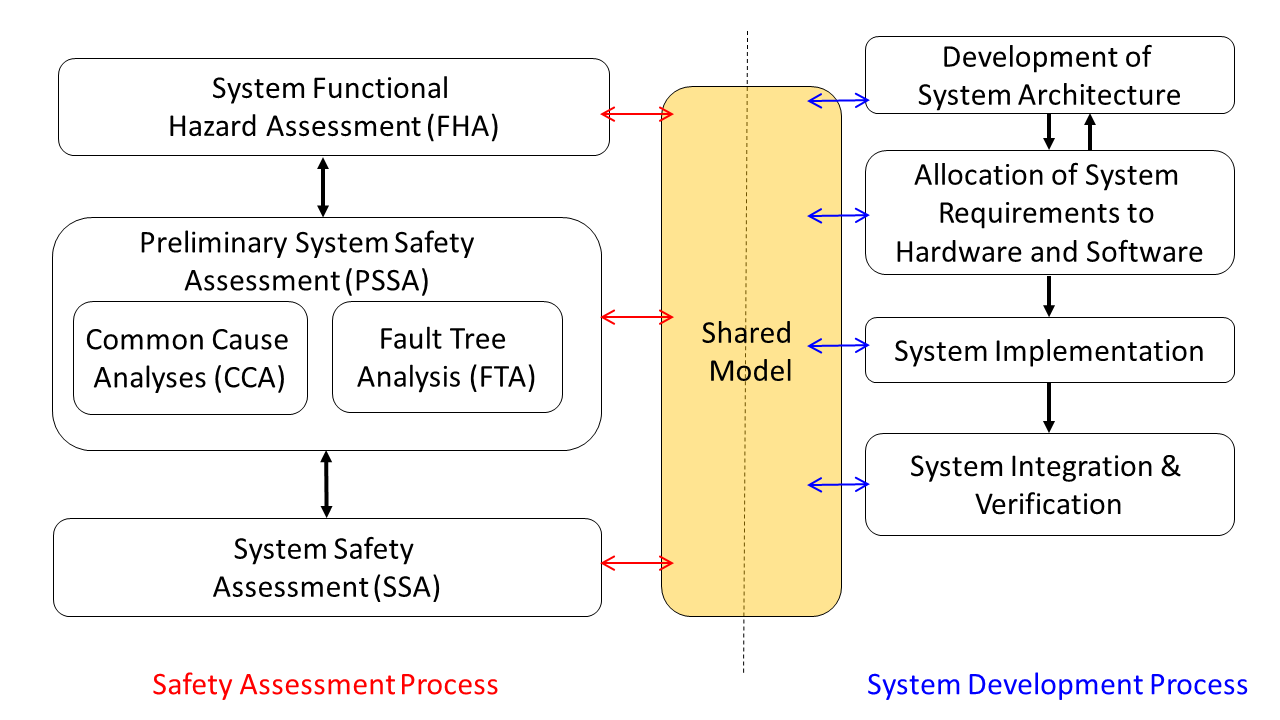
\includegraphics[trim=0 5 0 5,clip,width=0.85\textwidth]{images/process3.png}
	\caption{Use of the Shared System/Safety Model in the ARP4754A Safety Assessment Process}
	\label{fig:proposed_safety_process}
\end{figure}

%There are other tools purpose-built for safety analysis, including AltaRica~\cite{PROSVIRNOVA2013127}, smartIFlow~\cite{info8010007} and xSAP~\cite{DBLP:conf/tacas/BittnerBCCGGMMZ16}. These tools and their accompanying notations are separate from the system development model. Other tools extend existing system models, such as HiP-HOPS~\cite{CHEN201391} and the AADL Error Model Annex, Version 2 (EMV2)~\cite{EMV2}. EMV2 uses enumeration of faults in each component and explicit propagation of faulty behavior to perform error analysis. The required propagation relationships must be manually added to the system model and can become complex, leading to mistakes in the analysis.

%Alternatively, we wish to introduce a tool designed as an extension of AADL, an SAE approved modeling language. This tool will support model checking and perform the safety analysis by attaching faults to components and then utilize the proof mechanisms of a model checker to allow for behavioral propagation through the system model.  This allows users to reason about the evolution of faults over time, and produce counterexamples demonstrating how component faults lead to failures. Because of the relation of the safety analysis tool with a model checker, we wish to leverage the verification results to automatically generate safety assessment artifacts, such as fault trees and minimal cut sets.
%Our approach adapts the work of Joshi et. al~\cite{Joshi05:Dasc} to the AADL modeling language.  Stewart, et. al provide more information on the approach~\cite{Stewart17:IMBSA}, and the tool and relevant documentation can be found at: \small \url{https://github.com/loonwerks/AMASE/}. \normalsize


\section{Related Work}
The related work has two main focuses. The first is in regard to safety analysis tools and research and how the Safety Annex differs from related approaches. The second outlines related work in minimal cut set generation, probabilistic computations over fault trees, and tools that implement this research. 

\textbf{Safety Analysis Tools and Research:}
A model-based approach for safety analysis was proposed by Joshi et. al in \cite{Joshi05:Dasc, Joshi05:SafeComp, Joshi07:Hase}.  In this approach, a safety analysis system model (SASM) is the central artifact in the safety analysis process, and traditional safety analysis artifacts, such as fault trees, are automatically generated by tools that analyze the SASM.

The contents and structure of the SASM differ significantly across different conceptions of MBSA.  We can draw distinctions between approaches along several different axes.  The first is whether they propagate faults explicitly through user-defined propagations, which we call {\em failure logic modeling} (FLM) or through existing behavioral modeling, which we call {\em failure effect modeling} (FEM).  The next is whether models and notations are {\em purpose-built} for safety analysis vs. those that extend {\em existing system models} (ESM).

For FEM approaches, there are several additional dimensions.  One dimension involves whether {\em causal} or {\em non-causal} models are allowed.  Non-causal models allow simultaneous (in time) bi-directional %failure
error propagations, which allow more natural expression of some failure types (e.g. reverse flow within segments of a pipe), but are more difficult to analyze.  A final dimension involves whether analysis is {\em compositional} across layers of hierarchically-composed systems or {\em monolithic}.  Our approach is an extension of AADL (ESM), causal, compositional, mixed FLM/FEM approach.

Tools such as the AADL Error Model Annex, Version 2 (EMV2)~\cite{EMV2} and HiP-HOPS for EAST-ADL~\cite{CHEN201391} are {\em FLM}-based {\em ESM} approaches.  Given many possible faults, these explicitly defined propagation relationships require substantial user effort and become very complex.  In addition, it becomes the analyst's responsibility to determine whether faults can propagate; missing propagations lead to unsound analyses.  In the approach of this dissertation, propagations occur through system behaviors (defined by the nominal contracts) with no additional user effort. Furthermore, the interactions that cannot occur through behavioral propagation alone can be manually added as dependencies; this provides the \textit{mixed FEM/FLM} approach.

Closely related to our work is the model-based safety assessment toolset called COMPASS (Correctness, Modeling project and Performance of Aerospace Systems)~\cite{10.1007/978-3-642-04468-7_15}.  COMPASS is a mixed {\em FLM/FEM}-based, {\em causal} {\em compositional} tool suite that uses the SLIM language, which is based on a subset of AADL, for its input models~\cite{5185388, criticalembeddedsystems}. In SLIM, a nominal system model and the error model are developed separately and then transformed into an extended system model.  This extended model is automatically translated into input models for the NuSMV model checker~\cite{Cimatti2000, NuSMV}, MRMC (Markov Reward Model Checker)~\cite{Katoen:2005:MRM:1114692.1115230, MRMC}, and RAT (Requirements Analysis Tool)~\cite{RAT}. The safety analysis tool xSAP~\cite{DBLP:conf/tacas/BittnerBCCGGMMZ16} can be invoked in order to generate safety analysis artifacts such as fault trees and FMEA tables~\cite{compass30toolset}.  COMPASS is an impressive tool suite, but some of the features that make AADL suitable for SW/HW architecture specification: event and event-data ports, threads, and processes, appear to be missing, which means that the SLIM language may not be suitable as a general system design notation (ESM).

SmartIFlow~\cite{info8010007} is a {\em FEM}-based, {\em purpose-built}, {\em monolithic} {\em non-causal} safety analysis tool that describes components and their interactions using finite state machines and events. Verification is done through an explicit state model checker which returns sets of counterexamples for safety requirements in the presence of failures.  SmartIFlow allows {\em non-causal} models containing simultaneous (in time) bi-directional %failure
error propagations.  On the other hand, the tools do not yet appear to scale to industrial-sized problems, as mentioned by the authors: ``As current experience is based on models with limited size, there is still a long way to go to make this approach ready for application in an industrial context''~\cite{info8010007}.


The Safety Analysis and Modeling Language (SAML)~\cite{Gudemann:2010:FQQ:1909626.1909813} is a {\em FEM}-based, {\em purpose-built}, {\em monolithic} {\em causal} safety analysis language.  System models constructed in SAML can be used used for both qualitative and quantitative analyses. It allows for the combination of discrete probability distributions and non-determinism. The SAML model can be automatically imported into several analysis tools like NuSMV~\cite{Cimatti2000}, PRISM (Probabilistic Symbolic Model Checker)~\cite{CAV2011:KwNoPa}, or the MRMC probabilistic model checker~\cite{Katoen:2005:MRM:1114692.1115230}. 

AltaRica~\cite{PROSVIRNOVA2013127,BieberERTS2018} is a {\em FEM}-based, {\em purpose-built}, {\em monolithic} safety analysis language with several dialects.  There is one dialect of AltaRica which use dataflow ({\em causal}) semantics, while the most recent language update (AltaRica 3.0) uses non-causal semantics.  The dataflow dialect has substantial tool support, including the commercial Cecilia OCAS tool from Dassault~\cite{bieber2004safety}.  For this dialect the Safety assessment, fault tree generation, and functional verification can be performed with the aid of NuSMV model checking~\cite{symbAltaRica}. Failure states are defined throughout the system and flow variables are updated through the use of assertions~\cite{Bieber04safetyassessment}.  AltaRica 3.0 has support for simulation and Markov model generation through the OpenAltaRica (www.openaltarica.fr) tool suite.

\textbf{Minimal Cut Set Generation and Probabilistic Evaluations:}
Formal verification tools based on model checking have been used to automate the generation of safety analysis artifacts~\cite{bieber2002combination,schafer2003combining,bozzano2007symbolic,bozzano2003improving,volk2017fast,Joshi05:SafeComp,CAV2015:BoCiGrMa}; unfortunately, these methods are limited in the generation of MinCutSets. This limitation impacts scalability of the tools produced and readability of fault trees; often the results do not represent the hierarchical structure of the system and result in a two-level fault tree that is a 'mile wide and an inch deep.' Some research has been performed address these limitations and to generate hierarchical fault trees~\cite{CAV2015:BoCiGrMa, 10.1007/978-3-319-11936-6-7}, but this approach is not performed in a compositional way. In reality, fault trees are often manually generated due to the restrictions of automated approaches. 

The classical approach to \textit{fault tree analysis} (FTA) is two-fold: first the minimal cut sets are determined by either a bottom-up or a top-down approach and then probabilistic computations proceed using the MinCutSets~\cite{vesely1981fault,henley1996probabilistic,rausand2003system}. Due to scalability reasons in large systems, usually not all cut sets are considered; only the ones with lower cardinality (i.e. higher overall probability) are assessed~\cite{vesely1981fault,Bozzano:2010:DSA:1951720}. The representation of Boolean formulae as Binary Decision Diagrams (BDDs) was first formalized in the mid 1980s~\cite{bryant1986graph} and were extended to the representation of fault trees not many years later~\cite{rauzy1993new}. After this formalization, the BDD approach to FTA provided a new approach to safety analysis. The model is constructed using a BDD, then a second BDD (usually slightly restructured) is used to encode MinCutSets\cite{rauzy2008binary}. Probabilistic quantities are then assessed using either of these encodings. The hope was that this approach would provide `exact' probabilistic quantities of the top level event and not require the full MinCutSet generation to proceed. Unfortunately, due to the structure of BDDs, the worst case is exponential in size in terms of the number of variables~\cite{bryant1986graph,rauzy1993new,rauzy2008binary}. In industrial sized systems, this is not realistically useful. 

As the years continued, research was performed to encode the BDDs in more efficient ways and thus shrinking the size in order to address scalability; these are referred to as \textit{zero-suppressed} BDDs, or ZBDDs~\cite{minato2001zero}. While this helped to produce more scalable results than a pure BDD encoding, ZBDDs still suffered from scalability problems~\cite{matuzas2015dynamic, jung2008fast}. 

Some research has been introduced that attempted to address this problem by use of under and over approximation of the top-level probability during the minimal cut set computations~\cite{CAV2015:BoCiGrMa}. This allows for a converging limits on either side of the true probability. This provides valuable information even when all MinCutSets cannot be computed. Other research and tools have given the over-approximation as simply a few orders of magnitude higher than the under-approximation to account for the error term dropped during MinCutSet computations where only certain cardinalities are considered~\cite{symbAltaRica, bozzano2003improving, CHEN201391,Bozzano:2010:DSA:1951720}. 


